
\begin{frame}{Vienna: avoiding reinfection}
\begin{itemize}
\item scans through active directories for executables
\item ``marks'' infected executables in \myemph{file metadata}
\begin{itemize}
    \item could have checked for virus code --- but slow
\end{itemize}
\end{itemize}
\end{frame}

\begin{frame}{DOS last-written times}
\begin{itemize}
    \item 16-bit number for date; 16-bit number for time
\end{itemize}
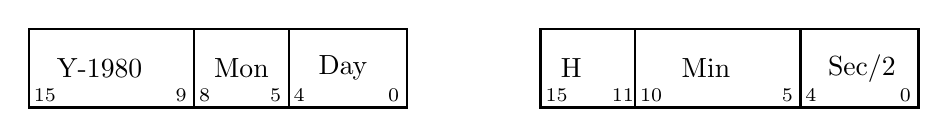
\begin{tikzpicture}
\tikzset{
    mylabel/.style={anchor=center},
    bitlabel/.style={font=\scriptsize,anchor=south west,inner sep=.5mm,text depth=.1mm},    
};
\begin{scope}[x=1.2cm]
\begin{scope}[thick]
    \draw (0, 0) rectangle (4, 1);
    \draw (0, 0) rectangle (1.75, 1);
    \node[bitlabel] at (0, 0) {15};
    \node[bitlabel] at (1.5, 0) {9};
    \draw (1.75, 0) rectangle (2.75, 1);
    \node[bitlabel] at (1.75, 0) {8};
    \node[bitlabel] at (2.5, 0) {5};
    \draw (2.75, 0) rectangle (4., 1);
    \node[bitlabel] at (2.75, 0) {4};
    \node[bitlabel] at (3.75, 0) {0};
\end{scope}
\node[mylabel] at (.75, 0.5) {Y-1980};
\node[mylabel] at (2.25, 0.5) {Mon};
\node[mylabel] at (3.325, 0.5) {Day};
\end{scope}

\begin{scope}[x=1.2cm,xshift=6.5cm]
\begin{scope}[thick]
    \draw (0, 0) rectangle (4, 1);
    \draw (0, 0) rectangle (1, 1);
    \node[bitlabel] at (0, 0) {15};
    \node[bitlabel] at (.7, 0) {11};
    \draw (1, 0) rectangle (2.75, 1);
    \node[bitlabel] at (1.0, 0) {10};
    \node[bitlabel] at (2.5, 0) {5};
    \draw (2.75, 0) rectangle (4., 1);
    \node[bitlabel] at (2.75, 0) {4};
    \node[bitlabel] at (3.75, 0) {0};
\end{scope}
\node[mylabel] at (.325, 0.5) {H};
\node[mylabel] at (1.75, 0.5) {Min};
\node[mylabel] at (3.4, 0.5) {Sec/2};
\end{scope}
\end{tikzpicture}
\begin{itemize}
    \item<2> Sec/2: 5 bits: range from 0--31
        \begin{itemize}
        \item corresponds to 0 to \textbf{62} seconds
        \end{itemize}
    \item<2> Vienna trick: set infected file times to \textbf{62} seconds
    \item<2> need to update times anyways --- hide tracks
\end{itemize}
\end{frame}

